% !Mode:: "TeX:UTF-8"
\chapter{行为级仿真,时序分析及性能验证}

通过前面几章,详细描述了整个分支预测框架的设计细节,以及相对于第一版架构做出的改进。本章主要介绍所有的工作实现后,如何从多个方面来评估设计带来的提升,首先介绍香山使用的评估环境,由于第二版设计还没有流片完成,且FPGA也还未成功运行,因此目前仍然是使用在服务器上用软件进行行为级仿真的方式来测试设计的正确性和性能。这种方式相比于最终的流片结果测试数据会有一定误差,但是通过和第一版代码使用相同行为级仿真的测试方法测出的结果来比较性能的提升也是有一定说服力的。然后介绍行业内认可度比较高的,测试整体性能的评估程序Coremark和SPEC 2006,最后介绍与整体性能或分支预测性能相关的一些评估指标,并解释选择这些指标的原因。之后通过对比第一版香山和第二版香山的实验结果进行统计对比,体现本文设计的有效性和带来的提升。

\section{开发工具与实验平台}

\subsection{Chisel}

Chisel (Constructing Hardware In a Scala Embedded Language) 是加州大学伯克利分校开发的一种开源硬件构造语言,它是一个建构在Scala语言\cite{scala}之上的领域专用语言 (DSL, Domain-Specific Language),不同于硬件设计领域传统的Verilog语言,Chisel建立在Scala这门高级编程语言之上。香山开发之所以选择使用Chisel语言,是因为它在具有更加高级的语言特性的同时又没有丢失底层电路设计的细节,它能够使用大量高级语言才有的特性,比如面向象编程和函数式编程的思想,能够从更高的抽象程度来描述硬件电路,实现更多Verilog难以完成的功能,极大的提高使用者的开发效率。

\subsection{差分测试框架}

在开发过程中,由于硬件电路非常复杂且难以调试,不同于软件开发有各种各样完善的调试工具,可以下断点追函数调用等,且由于仿真速度的限制,运行一次测试的时间也比普通的软件开发慢很多。因此香山团队开发了一套差分测试框架,如图\ref{fig:figure64}所示, 即使用一个可以认为是实现正确的指令集的模拟器NEMU\cite{nemu},和硬件设计的仿真同时运行,并以NEMU为参考,在指令提交时比较两者的寄存器堆中的值是否相同,来判断硬件设计运行时有没有出现指令执行结果错误的情况,当发现比对结果不同时,立马中断仿真,并且输出相关的处理器内部状态,以此来提高发现和定位问题的效率。当然由于分支预测的特殊性,一些只影响分支预测准确率的功能实现错误时,例如分支历史更新逻辑有问题,这种情况下只会影响性能,程序依然能够正确的执行完毕。因此这种错误使用差分框架难以发现。

\begin{figure}[htb]
	\centering
	\setlength\tabcolsep{3pt}  % 同一行中的图片间隔
	\vspace{5pt} % 图片上部的空白,如果太小的话,图片顶部会与正文内容十分接近
	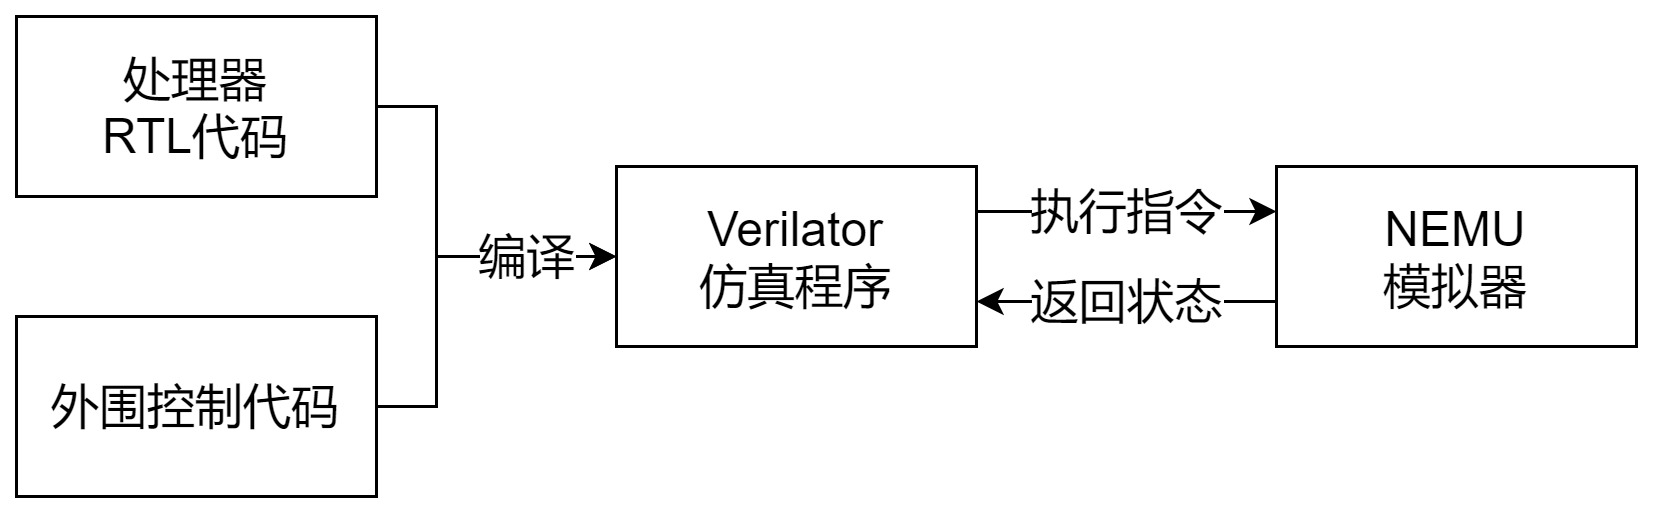
\includegraphics[width=1\textwidth]{diff.jpg}
	\caption{差分测试框架,NEMU和仿真程序同时运行,比较运行结果}
	\label{fig:figure64}
\end{figure}

\subsection{Verilator}

Verilator\cite{verilator}是一款开源免费的Verilog/System Verilog仿真器,可用于将Verilog代码转换成C++代码,在服务器上通过运行软件程序对硬件设计进行行为级仿真验证。相比于类似的另一种仿真工具VCS\cite{vcs},由于Verilator仿真的电路只有0和1两个状态,不同于VCS有0、1、X、Z四个状态,因此在运行处理器这种大型的电路仿真时,它仿真运行的速度会比VCS更快。但是毕竟处理器整体的RTL设计过于复杂,因此它的仿真速度在有跑SPEC这类大型测试程序时速度依然是一个关键的问题。相比于差分测试框架中纯软件的指令集模拟器NEMU来说,运行速度差了好几个数量级。

\section{验证环境与评估指标}

\subsection{验证环境}

硬件部分CPU使用的是AMD EPYC 7742 128核,操作系统是Ubuntu 20.04.3 LTS。服务器上对设计进行行为级仿真来进行验证与评估,首先通过脚本将Chisel编写的RTL代码编译成功能相同的Verilog代码,然后再用verilator将其转变为仿真用的可执行文件,在电脑上运行行为级仿真,模拟电路运行时的状态。

通过差分测试框架,NEMU会和需要仿真的电路同时运行,由于NEMU执行指令的速度速度比仿真程序快了好几个数量级,且占用资源极少,因此并不会对仿真需要运行的时间带来太大的影响,且可以随时监控程序仿真有没有出现指令执行错误的情况,及时中断仿真并报告出错现场。

使用的测试程序有很多,通常一些小的改动和简单测试,会运行Coremark,这是由EEMBC发布的测试处理器核心性能的一项基准测试程序,
程序使用C语言写成,主要功能包含如下四类运算法则:

\begin{enumerate}
	\item 数学矩阵操作(普通矩阵运算)
	\item 列举(寻找并排序)
	\item 状态机(用来确定输入流中是否包含有效数字)
	\item CRC(循环冗余校验)
\end{enumerate}

Coremark程序比较小,运行一次需要的时间很短,但是为了能够让处理器充分运行起来,例如给分支预测一些训练的时间,因此在跑Coremark时通常都会连续执行很多次迭代运行,例如迭代运行100次。通过运行Coremark,在初步的开发时,一些很容易触发的,比较明显的bug就能够很快的找到。并且由于运行一次的时间很短,因此修改bug时可以快速迭代。

此外在需要更多的测试程序,想要测试更多复杂的情况时,通常会通过运行SPEC 2006\cite{spec-2006}来测试电路性能。SPEC 2006是SPEC (Standard Performance Evaluation Corporation) 组织推出的CPU系统评估软件,是业内比较权威的性能参考指标,SPEC 2006中包含有SPECint 2006和SPECfp 2006两个基准,SPECint 2006中包含12个不同的基准测试,SPECfp 2006中包含19种不同的基准测试。SPEC 2006和SPEC 2017也是香山发布时公开的最主要的性能数据,大量的处理器相关研究都会以这两个测试的得分来评估性能。

除此之外还有其他的测试程序,例如Dhrystone\cite{dhrystone}、SPEC 2017,以及一些简单小程序的集合Microbench。针对某些特定的模块,也会有针对特定功能的单元测试程序。

% 找耀阳师兄要引用

值得一提的是由于香山整个项目的设计非常复杂,因此在使用Verilator进行行为级仿真时速度非常慢,在运行Coremark这类程序时所花费的时间还可以承受,但是当需要运行SPEC测试时,所需要花费的时间就要按月计算。因此香山团队开发了一套基于checkpoint的测试方法。其主要思路在于通过神经网络训练,找到一个程序中最具有代表性的片段,并给出各自的权值,能够保证运行完这些片段之后将其对应的性能数据乘以权值的和尽可能接近完成的测试程序。这样的话就不用运行完整的测试程序,只要运行一些程序片段即可。且因为一个程序被切分为许多片段,因此可以通过并行运行这些片段来进一步缩短测试运行的时间。

由于有一个运行速度极快的指令集模拟器NEMU,因此可以先使用NEMU来训练切片,验证片段的准确性,然后再使用Verilator仿真运行这些程序片段,真正验证设计的性能。

由于checkpoint在恢复时只能够恢复内存和寄存器,像FTB这类SRAM无法完全恢复,因此在真正的测试片段运行前,需要运行测试片段前的一小部分程序,为整个流水线做warmup,经过一段时间的训练后再开始运行正式的测试片段。通过这种技术,可以在几周内就得到一次完整的SPEC测试数据,极大提升了迭代效率。

由于运行一次完整的SPEC 2006测试,即使使用了checkpoint技术,也需要几周的时间。因此为了更快的得到测试的性能结果,本文的性能评估一节中,只选取了SPEC 2006的部分有代表性的测试点进行测试。

通过在代码中添加各种各样的性能计数器。在测试程序执行完毕后,可以通过查看性能计数器的结果,来判断分支预测部分的工作情况,并通过跟香山第一版的架构进行比对,来验证第二版设计的性能提升。

\subsection{验证评估指标}

本文的评估指标有:

\begin{enumerate}
	\item IPC (Instructions Per Cycle)。即每周期有多少条指令提交,用总的指令数除以程序运行的总周期数得到。这是评估整个处理器架构性能的关键指标,IPC越高,说明单位时间内处理器能够执行的指令越多,性能越好,且IPC以周期数为衡量指标,可以很好的排除频率的影响。
	\item 分支预测准确率。即用预测正确的分支数量除以总分支数量,即可得到分支预测准确率,相反的,用预测错误的分支数量除以总分支数量,得到的就是分支误预测率,分支预测准确率加分支误预测率等于1。分支预测准确率可以比较直观的看出分支预测的性能。在现代处理器的分支预测设计下,基本上预测准确率能够达到90\%以上。
	\item MPKI (Misprediction Per KiloInstructions)。代表在整个测试程序中每1000条指令中误预测指令的数量。也是衡量分支预测性能的一个重要指标。与分支预测准确率不同的是,MPKI除了考虑了分支指令以外,将所有的指令都纳入了考虑的范围内。通常情况下希望MPKI越低越好,但是导致MPKI低的原因不只有分支预测准确率高,一个分支指令占总指令比较低的程序也有可能达到很低的MPKI,即使它的预测准确率较低。使用MPKI评估分支预测性能的原因是现在分支预测在很多情况下的准确率都已经非常高,一些应用甚至准确率能够达到99\%,这种情况下再对比分支预测准确率的差距就不是很明显了。此外使用MPKI也能够更直观的看出误预测分支指令在整个程序中的占比,更容易评估误预测带来的penalty。
	\item FTB命中率。这是用于评估FTB的一个主要指标,在第二版的前端设计中,主要靠FTB来识别并给出分支指令的相关信息,如果FTB没有命中,分支预测就无从谈起,因此FTB的命中率也是影响分支预测准确率的一个重大因素。
	% \item 前端气泡数量?
	\item 频率。通过计算IPC,能够得知处理器整体架构每周期有多少条指令提交,除了提升IPC能够提高处理器的性能之外,提升频率也是一个重要的途径。频率越高,代表处理器每周期的时间越短,相同时间内包含更多周期,因此在相同IPC的情况下,频率越高,单位时间内处理器能够执行的指令数量也越多,总体性能越高。
\end{enumerate}

\section{评估结果分析}

本节将根据上一节提出的评估指标,来对SPEC 2006的部分测试成果进行分析。主要用于对比的是香山处理器第一版和第二版,因为香山第二版主要是在第一版的基础上进行迭代优化,希望能够进一步的提升性能。

图\ref{fig:figure61}是运行占80\%权重的SPEC 2006部分测试程序片段后,第一版和第二版的IPC数据对比,可以看出第二版相比于第一版的性能,大部分的程序IPC都有了提升,总体的IPC平均提升了30.96\%。当然IPC提升的原因有很多,第二版架构相比于第一版也不只是重构分支预测和解耦了前端。因此IPC并不能够直观的反应分支预测部分性能的提升,但是解耦前端消除的气泡带来的性能提升依然占其中一部分比例。而由于两个版本架构解耦前后的前端差距过大,因此没有办法很好的控制变量,精准的测试出解耦带来的性能提升。

% 9.32 -18.4 17.6 67.05 28.57 58.57 51.19

\begin{figure}[htb]
	\centering
	\setlength\tabcolsep{3pt}  % 同一行中的图片间隔
	\vspace{5pt} % 图片上部的空白,如果太小的话,图片顶部会与正文内容十分接近
	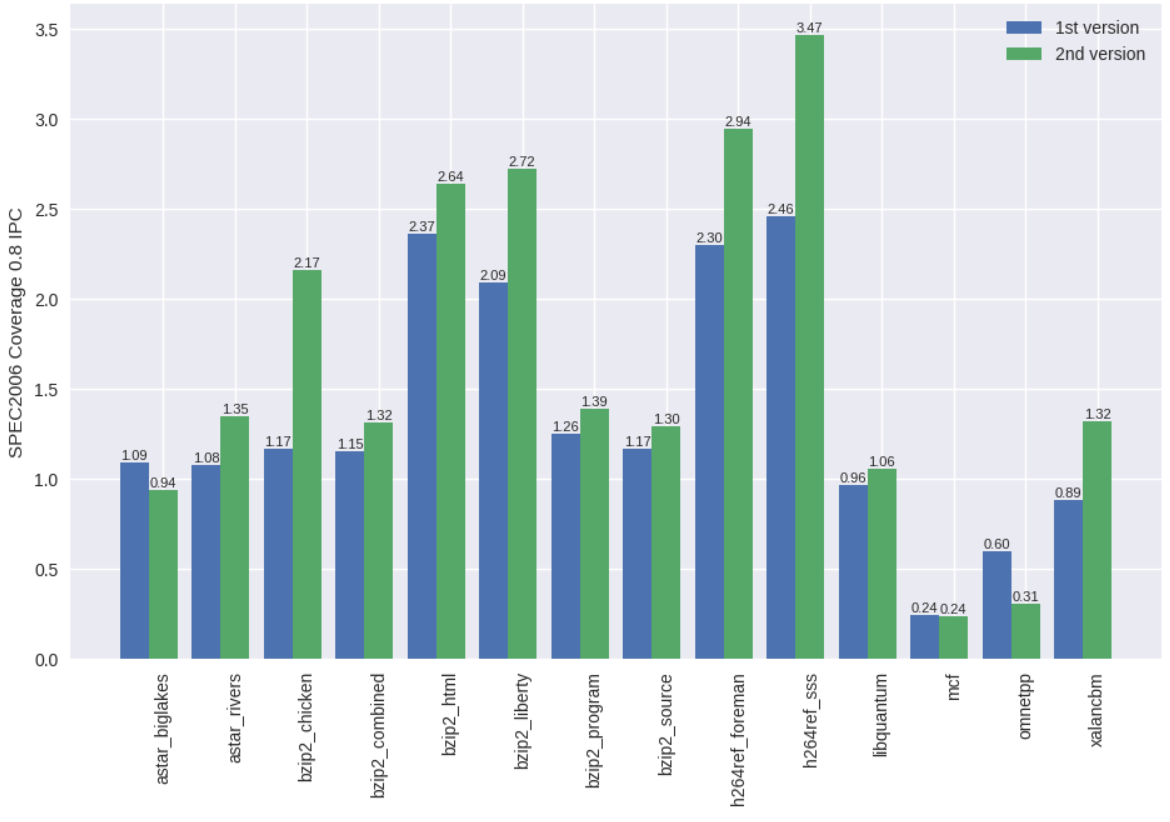
\includegraphics[width=0.9\textwidth]{ipc.png}
	\caption{SPEC2006 coverage 0.8 部分检查点IPC对比}
	\label{fig:figure61}
\end{figure}

图\ref{fig:figure64}和图\ref{fig:figure62}分别是运行占80\%权重的SPEC 2006部分测试程序片段后,第一版和第二版的分支预测准确率和MPKI对比。可以看出相比于第一版设计,第二版设计的平均MPKI降低了0.6\%,平均MPKI降低了1.13。分支预测性能变化的主要因素,主要有在第二版中使用了更加准确的单条指令的分支历史,并且增加了FTB使用的SRAM的容量,会对分支预测准确率有一定的正面影响,但是为了优化逻辑电路的延时,提高最终的频率,因此分支预测依然在很多方面做了性能上的妥协,例如减少了TAGE预测表的数量,最终各种因素综合,得到了最终的性能变化。

\begin{figure}[htb]
	\centering
	\setlength\tabcolsep{3pt}  % 同一行中的图片间隔
	\vspace{5pt} % 图片上部的空白,如果太小的话,图片顶部会与正文内容十分接近
	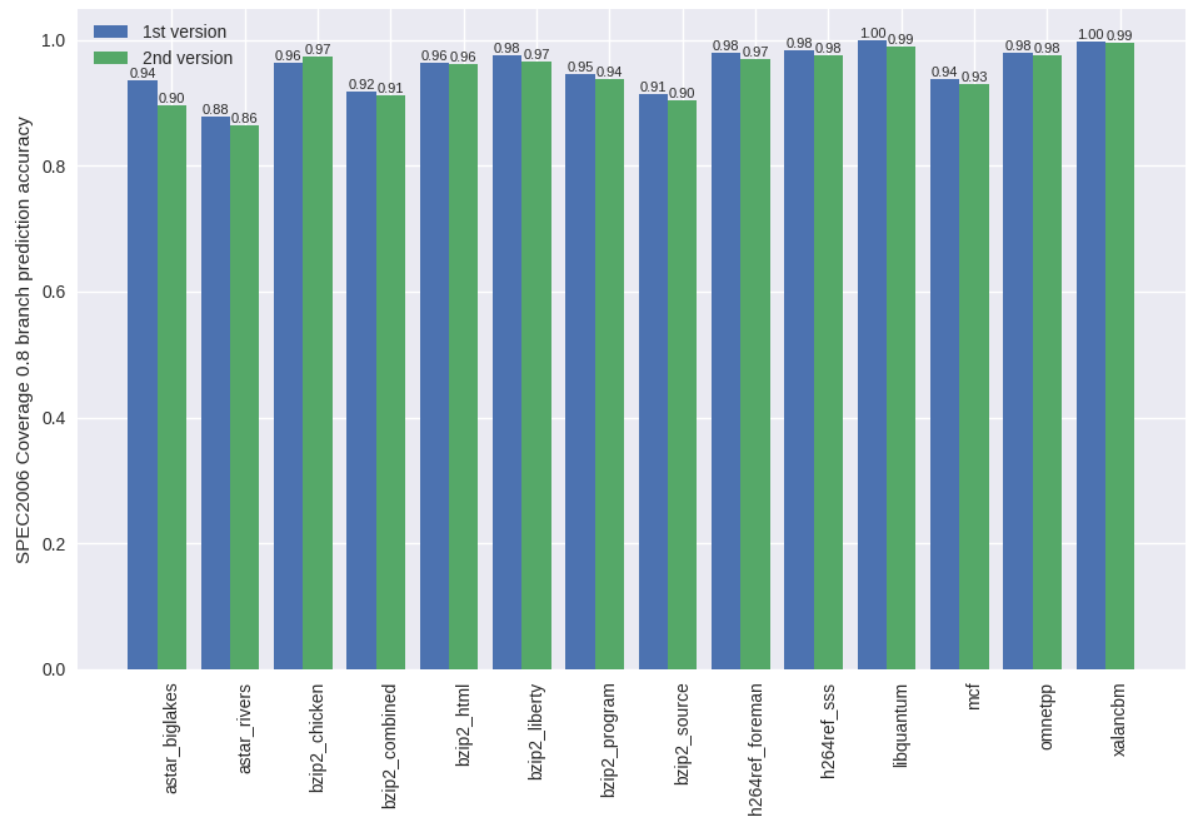
\includegraphics[width=1\textwidth]{accuracy.png}
	\caption{SPEC2006 coverage 0.8 部分检查点分支预测准确率对比}
	\label{fig:figure64}
\end{figure}

% 13.05 -39.61 40.68 86.36 20.68 -1.6 


\begin{figure}[htb]
	\centering
	\setlength\tabcolsep{3pt}  % 同一行中的图片间隔
	\vspace{5pt} % 图片上部的空白,如果太小的话,图片顶部会与正文内容十分接近
	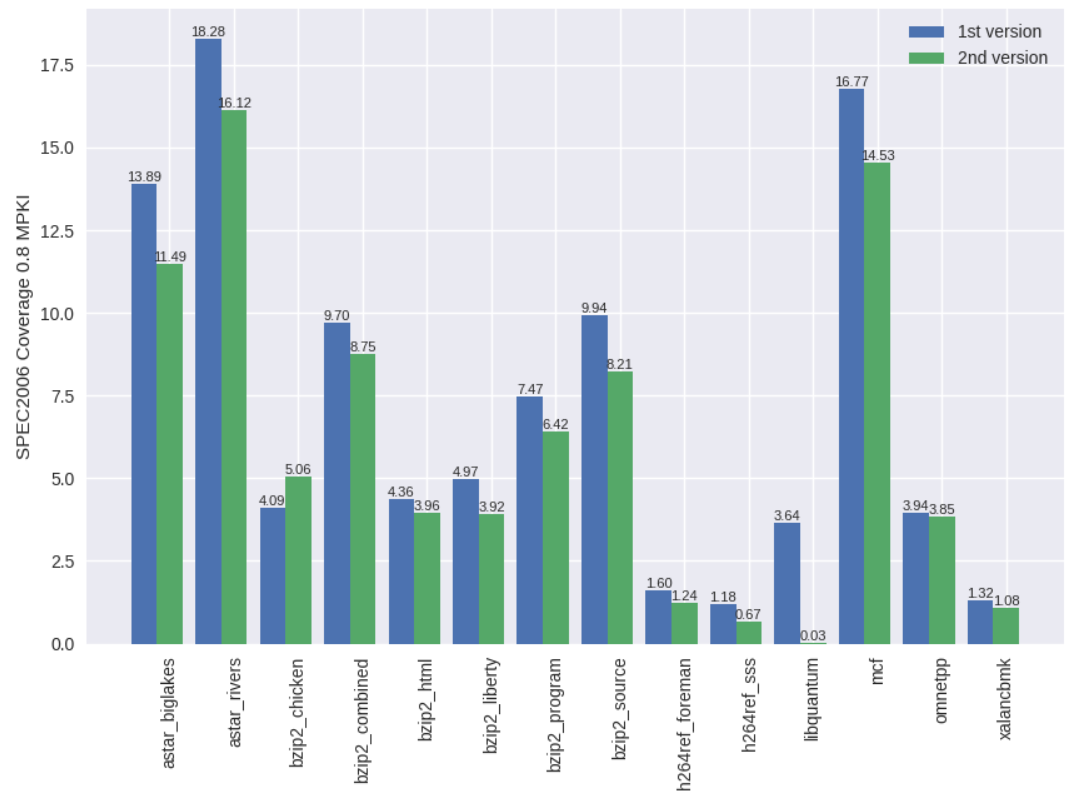
\includegraphics[width=1\textwidth]{mpki.png}
	\caption{SPEC2006 coverage 0.8 部分检查点MPKI对比}
	\label{fig:figure62}
\end{figure}

图\ref{fig:figure63}是在SRAM大小相同的情况下,运行占80\%权重的SPEC 2006部分测试程序片段后,第一版和第二版BTB和FTB的命中率对比,可以看出相比于BTB,FTB的命中率平均降低了3.1\%,这主要是由于未跳转分支指令在跳转前不会被存入FTB所带来的。在第二版分支预测设计中,FTB使用了比第一版BTB更大的SRAM,一定程度上减轻了FTB命中率下降的问题,但是这个问题依然存在。后续如何对其进行优化也是一个值得探讨的课题。

% 3.37 2.86 2.06 2.27 4 4.05


\begin{figure}[htb]
	\centering
	\setlength\tabcolsep{3pt}  % 同一行中的图片间隔
	\vspace{5pt} % 图片上部的空白,如果太小的话,图片顶部会与正文内容十分接近
	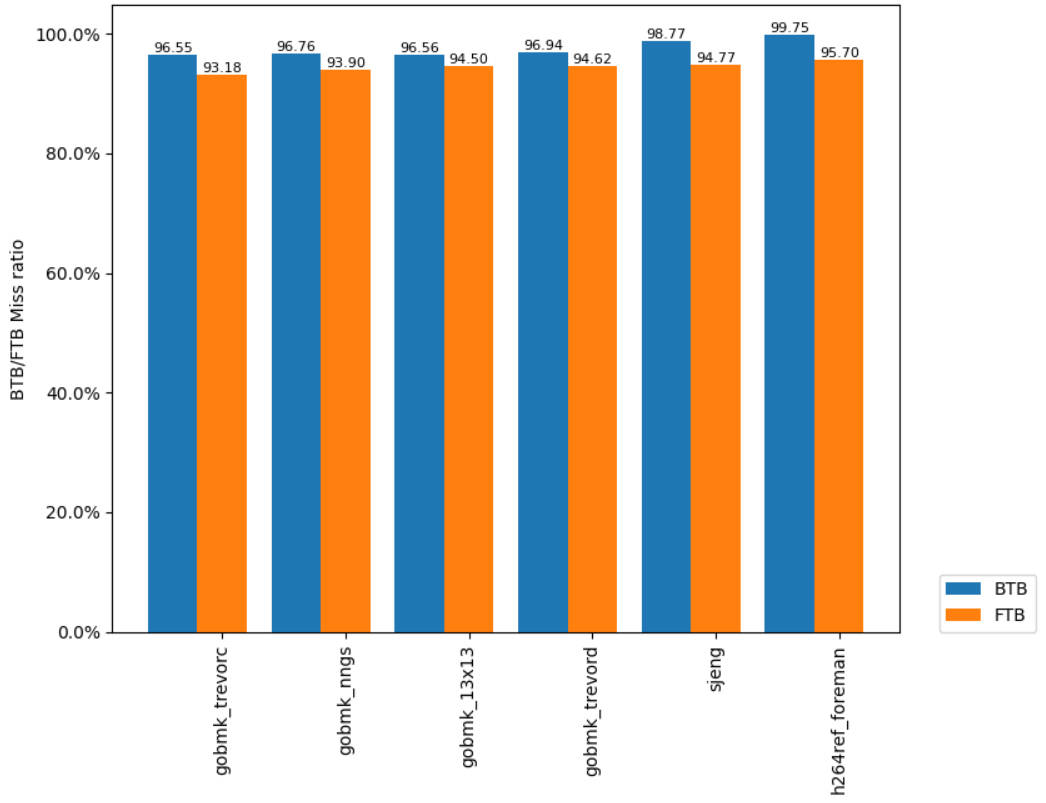
\includegraphics[width=1\textwidth]{ftb-hit-data.jpg}
	\caption{SPEC2006 coverage 0.8 部分检查点FTB/BTB命中率对比}
	\label{fig:figure63}
\end{figure}

% \begin{table}[]
%     \caption{两版架构频率对比}
%     \label{tb:table1}
%     \centering
%     \begin{tabular}{|c|c|c|}
%         \hline
%         版本   & 工艺   & 主频   \\ \hline
%         第一版 & 28nm & 1.3GHz \\ \hline
%         第一版 & 14nm & 1.8GHz \\ \hline
%         第二版 & 14nm & 2.0GHz \\ \hline
%     \end{tabular}
% \end{table}

频率方面是第一版和第二版架构种前端最主要的提升。香山第一版架构流片时使用的是28nm的制作工艺,主频能够达到1.3GHz,而用14nm的工艺库评估香山第一版,最高能够达到1,8GHz的主频。香山第二版架构流片使用的是14nm工艺,主频能够达到2GHz。如表\ref{tb:table3}所示。在第一版的基础上,通过重构分支预测部件,降低预测宽度,修改预测算法的实现等优化后,第二版架构的总体时序评估结果,在相同工艺库下,能够做到的主频相比于第一版提升了11\%。

~\\

\begin{table}[!h]
	\caption{香山第一版和第二版频率对比}
	\label{tb:table3}
	\centering
	\begin{tabular}{|c|c|c|}
		\hline
		架构版本   & 工艺库   & 主频   \\ \hline
		第一版 & 28nm & 1.3GHz \\ \hline
		第一版 & 14nm & 1.8GHz \\ \hline
		第二版 & 14nm & 2.0GHz \\ \hline
	\end{tabular}
\end{table}


\section{本章小结}

本章主要介绍了整个项目在进行测试和性能评估时使用的工具和方法,并从多个角度分析了第二版架构相比于第一版架构带来的改变。这也是在频率和性能之间不断进行权衡比较的结果,相比于第一版架构,第二版架构分支预测的性能有小幅的提升,而最终的总体性能,以及能够达到的最终流片频率均有较大的提升。